In this chapter some theoretical models, which are applicable for description 
of proton-induced spallation reactions will be discussed. 
According to hypothesis of Serber \cite{Serber}, such a reaction proceeds in two steps. 
The first step is a cascade of binary collisions 
among the constituents of the target nucleus, induced by the impinging projectile. 
This stage lasts a few fm/c.
Elastic and inelastic interactions lead to distribution of the excitation among the target nucleons and creation of resonances (mainly deltas). 
Decay of resonances is a source of pions, which additionally contribute to the cascade of interactions. Those of nucleons and pions, which energies exceed their separation energies can be emitted. Also the complex objects like the H and He isotopes (and even heavier composite particles) 
can appear in this stage of reaction. 

The hypothesis of Serber assumes furthermore that after cascade of emissions of fast particles the
excited remnant of the target nucleus is left in its thermal equilibrium.  

The second stage of the reaction consists in de-excitation of this remnant nucleus by various processes like 
particle evaporation, (multi-) fragmentation, asymmetric and symmetric fission. 
These processes are a source of single nucleons, light composite nuclear aggregates called the light charge particles (LCP), Intermediate Mass Fragments (IMF) of the mass number $A > $ 4 but lighter than fission fragments and  heavy residues.

In general the shapes of experimental spectra of spallation reactions can be described with the models adopting such two step scenario of reaction.
However, the low precision of the theoretical reproduction of the data induces the need for looking for more complicated or quite different hypotheses 
of the reaction scenarios. For example there are models, which assume the three steps of the reaction.
The intermediate stage called a pre-equilibrium stage is assumed between the cascade and the full thermal equilibration of the system. 

In the next sections, a most commonly used models of the first and the second stage of reactions will be described.

\section{Models of the first stage reactions}

Among the models used to describe the dynamics of the proton target nucleus collision (i.e. first stage of reaction) are 
INCL \cite{INCLCugnon1981,INCLboudard2002intranuclear,INCLboudard2004new,INCLboudard2013new,INCLMancusi2014}, 
GiBUU\cite{GiBUUBuss2012}, UrQMD\cite{UrQMDBASS1998,UrQMDBleicher1999}, 
JAM\cite{JAM_NARA1999}, 
INC by Bertini \cite{Bertini1963,Bertini1969}, 
CEM \cite{CEM_GUDIMA1983}, 
and ISABEL \cite{Isabel_Yariv1979,Isabel_Yariv1981}. 
Some of the them were created especially to study the spallation reactions (INCL, INC). Others try to describe 
in general the collisions of nuclear objects (e.g. the heavy ion collisions) and broad diversity of fundamental 
nuclear processes (GiBUU, UrQMD).

%Here the most popular of them will be discussed.

\subsection{Intranuclear cascade models - INC}

In the simplest approximation the proceeding of the first step of reaction - the intranuclear cascade (INC) 
can be imagined as collisions of the free nucleons, pions and other particles embedded in the volume of the target nucleus. 
Individual collisions take place if predefined conditions are fulfilled. The excitation of $\Delta$ resonance is one 
of possible effects of interaction of two nucleons or nucleon and pion. When $\Delta$ de-excites the pion is created. 
Particles, which gained enough energy are emitted from the nucleus but those whose kinetic energy is lower than 
their separation energy are reflected at the nuclear surface back into the nucleus. Such simplified picture of intranuclear 
reaction is presented in fig. \ref{INCLsch}.

\begin{figure}[!hbt]
	\centering
	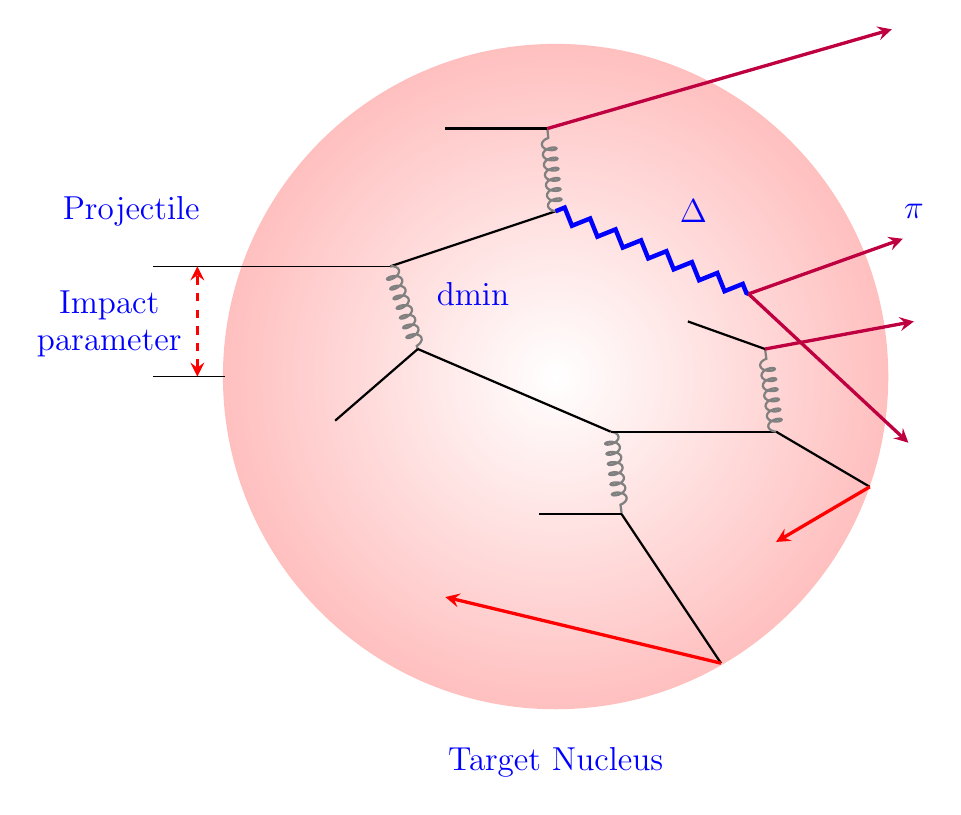
\begin{tikzpicture}[scale=0.7]
		
		\node[circle,outer color=pink!100!black,inner color=white,minimum width=8.45cm] (radial) at (0,0) {};
		\proton{-7.7,2};
		\proton{-2.3,4.5}
		\neutron{-4.3,-1};
		\proton{2.1,1.1}
		\pion{6.5,2.5}
		\proton{-0.6,-2.5};
		%\draw[ultra thick] (0,0) circle (6 cm);
		\draw[blue](2.5,3) node {\large $\Delta$};
		\draw[blue](-1.5,1.5) node {\large dmin};
		\draw[blue](6.5,3) node {\large $\pi$};
		\draw[blue](-7.7,3) node {\large Projectile};
		\draw[blue](-8.1,1.3) node {\large Impact};
		\draw[blue](-8.1,0.6) node {\large parameter};
		\draw[blue](0,-7) node {\large Target Nucleus};
		\draw [-](-7.3,2) --(-3,2);
		\draw [<->,>=stealth,very thick,color=red,dashed](-6.5,0) --(-6.5,2);
		\draw [-](-7.3,0) --(-6,0);
		\draw [-,thick](-3,2) --(0,3);
		\draw [color=gray,thick,decorate,decoration={coil,segment length=1.3mm, amplitude=0.9mm}](0,3) --(-0.15,4.5);
		\draw [-,thick](-2,4.5) --(-0.15,4.5);
		\draw [->,>=stealth,very thick,color=purple](-0.15,4.5) --(6.1,6.3);
		\draw [decorate,decoration={zigzag},ultra thick,color=blue](0,3) --(3.5,1.5);
		\draw [->,>=stealth,very thick,color=purple](3.5,1.5) --(6.3,2.5);
		\draw [->,>=stealth,very thick,color=purple](3.5,1.5) --(6.4,-1.2);
		\draw [color=gray,thick,decorate,decoration={coil,segment length=1.3mm, amplitude=0.9mm}](-3,2) --(-2.5,0.5);
		\draw [-,thick](-4,-0.8) --(-2.5,0.5); 
		\draw [-,thick](-2.5,0.5) --(1,-1);
		\draw [color=gray,thick,decorate,decoration={coil,segment length=1.3mm, amplitude=0.9mm}](1,-1) --(1.2,-2.5);
		\draw [-,thick](-0.3,-2.5) --(1.2,-2.5);
		\draw [-,thick](1.2,-2.5) --(3,-5.2);
		\draw [->,>=stealth,very thick,color=red](3,-5.2) --(-2,-4);
		\draw [-,thick](1,-1) --(4,-1);
		\draw [color=gray,thick,decorate,decoration={coil,segment length=1.3mm, amplitude=0.9mm}](4,-1) --(3.8,0.5);
		\draw [-,thick](2.4,1) --(3.8,0.5);
		\draw [->,>=stealth,very thick,color=purple](3.8,0.5) --(6.5,1);
		\draw [-,thick](4,-1) --(5.7,-2);
		\draw [->,>=stealth,very thick,color=red](5.7,-2) --(4,-3);
	\end{tikzpicture}
	\caption{Schematic explanation of the proceeding of the intranuclear cascade (INC). For details see text.}
	\label{INCLsch}
\end{figure}

%The models which assume, that the interactions of high-energy particles with the nucleus can be represented by free nucleon-nucleon and nucleon-pion collisions inside %the nucleus are called intranuclear cascade models. 
The first model of this type has been created by Bertini in 1963 \cite{Bertini1963,Bertini1969}. 
Later, this conception was used also in other codes, e.g. by Yariv in his ISABEL code \cite{Isabel_Yariv1979,Isabel_Yariv1981}. 
In the 80's and 90's, the several versions of INC model were developed by Cugnon et al.      \cite{INCLCugnon1981,INCLboudard2002intranuclear,INCLboudard2004new,INCLboudard2013new}. 
Model of Cugnon was called Intranuclear Cascade Li\`ege - INCL. Its latest version, utilized in this thesis, is INCL++5.6 \cite{INCLMancusi2014}.

INCL++ is most advanced among the models which utilize the assumption of the target nucleus as a Fermi gas of free nucleons kept in the nuclear potential well.
It this work it is used both as one of the theoretical models confronted with the experimental data as well as reliable event generator used for simulation of 
response of detection system.
Thus, it is described here in more details as the best example of the family of semi-classical INC models.  

% In this thesis, INCL++ was used for the validation of different proton-induced reactions. 
% Since the INC models are very similar to each other only the most advanced of them, 
% i.e. INCL4.6 (INCL++) is described here. Please note that INCL4.6 \cite{INCLboudard2013new} 
% is not identical with INCL++ \cite{INCLMancusi2014}. Text from ref\cite{INCLMancusi2014} 
% :"The physics of the new code is substantially equivalent to the reference FORTRAN77 version INCL4.6 
% for nucleon- and pion-induced reactions; the few minor differences will be highlighted in Sec. IIA". 
% The  INCL++ is also included in Geant4 \cite{Geant_AGOSTINELLI2003250} 
% code which is a well-accepted simulation code for various applications in high energy, 
% space and radiation, as well as in medical fields. In figure \ref{INCLsch} 
% the main features of INCL are represented.

\subsubsection{Features of INCL model}\label{FeaOFINCL}

The most important assumptions used in INCL++ model are as follows:

\begin{enumerate}[label=(\roman*)] 
	
	\item Target nucleus is treated as Fermi gas of protons and neutrons embedded in the potential well;
	\item Initial positions of nucleons are stochastically selected inside the sphere of the radius dependent on the mass number $A$ 
	and the selected density profile;
	\item Initial momenta of nucleons are as well randomly distributed inside the Fermi momentum sphere;	
	\item Nucleons move inside the nucleus along straight trajectories until two of them collide 
	or until one nucleon reaches the nucleus surface, where it can be transmitted or reflected (shown in figure \ref{INCLsch}).
	\item Collision takes place when the distance between two nucleons is smaller than $d_{min}$ which is given by:
	\begin{equation}
		d_{min}\leq\sqrt{\sigma_{tot}/\pi}
	\end{equation}
	where $\sigma_{tot}$ is the free space total nucleon-nucleon cross-section;	
	\item Nucleons are divided into participants (these which take part in the collision) and spectators (not collided). Spectator cannot be emitted; 
	\item Pauli blocking is checked both during creation of initial phase-space distribution of nucleons as well as for final state of each collision; 
    \item Relativistic kinematics is used in this model.
\end{enumerate}


\subsubsection{Construction of target nucleus}\label{TargetNucleus}
The spatial distribution $\rho (r)$ of nucleons inside the target nucleus is prepared according 
to a Saxon-Woods formula:
\begin{equation}
	\rho (r)= \begin{cases} \frac{\rho_{0}}{1+\exp(\frac{r-R_{0}}{a})} &  r \leq R_{max}\\ 
		0 &  r> R_{max} \end{cases} 
\end{equation}
where $R_{max}=r_{int} + R_{0} + 8a$ and $r_{int}=(\sigma_{NN}^{tot}/\pi)^\frac{1}{2}$. 
The $\sigma_{NN}^{tot}$ is the the free space total  nucleon-nucleon cross-section.

The $R_{0}$ and $a$ values are taken from electron scattering measurements for $Al$ to $U$ target nuclei and parametrized as below. 

\begin{align}
	R_{0} &=(2.7545*10^{-4}A_{T}+1.063)A_{T}^{1/3}\\
	a &=0.510 + 1.63 *10^{-4}A_{T}
\end{align}

$A_T$ is the mass number of the target nucleus.

The initial position and momentum of any target nucleon are generated as follows. First momentum $p$ is taken randomly from a sphere of radius $P_{F}$. 
Then $R(p)$ corresponding to  momentum $p$ is calculated by equation \ref{prp}. After that the position $r$ is randomly selected from the sphere of radius $R(p)$.

\begin{align}
	\left(\frac{p}{P_{F}}\right)^{3}&=-\frac{4\pi}{3A_{T}}\int_{0}^{R(p)}\frac{d\rho(r)}{dr}r^{3}dr,\label{prp}
\end{align}

For more details please, refer to \cite{INCLboudard2002intranuclear}.

\subsubsection{Potentials}

In the INCL++ model both the nuclear as well as the Coulomb potentials for nucleons and pions are taken into account.
Potentials for $\Delta$ particles are neglected.

Particles of the target nucleus are kept inside a potential well which approximates the mean nuclear potential.
The value of the nuclear potential for nucleons is dependent on their actual energy. The dependence of the potential 
on the isospin of the nucleon is kept as well. 

The energy and isospin dependent potential for nucleons is calculated according to formula \ref{Epoten}:

\begin{equation}\label{Epoten}
	V^{i}(E)= \begin{cases} V_{0}^{i}-\alpha\left(E-E_F^{i}\right) &  E \leq E_{0} \\ 
		0 &  E > E_{0} \end{cases} 
\end{equation}
In this equation superscript $i$ stands for proton ($i=p$) or neutron ($i=n$).
The parameter $\alpha$ of formula \ref{Epoten} is fixed and equal to 0.23, where energy E of nucleon of momentum $k$ can be calculated by:
\begin{align}
	E=\frac{\hbar^2k^2}{2M}+V_{0}^{i}(E) \label{energy}
\end{align}

The deepness of the potential $V_{0}^{i}$ is calculated from 
the Koopman's theorem \cite{KOOPMANS1934104}: 

\begin{equation}\label{V0}
	V_0^i = S_i + T_F^{i}
\end{equation}

where the appropriate quantities of separation energies $S_i$ are taken from experiments \cite{WAPSTRA198555}. 
The kinetic energy $T_F^{i}$ of the particle $i$ ($i = p$ for proton or $ = n$ for neutron) is related to its Fermi momentum $k_F^i$ which is different for proton and neutron and given by:
\begin{equation}\label{FKE}
	T_F^{i}=\frac{(\hbar k_F^i)^2}{2M}
\end{equation}

where $M$ is the mass of nucleon and $\hbar$ is the reduced Planck constant. 

The limiting value of $E_{0}$ above, at which the nuclear potential for nucleons vanishes is equal to:

\begin{equation}\label{E0}
E_0 = \frac{V_0^i}{\alpha} + T_F^i
\end{equation}
  
where $\alpha$  is a parameter having value 0.23. 
The values of the energy independent potentials for pions are distinguished according to their third component of isospin $\tau_3$. They are energy independent.
Potential for individual pion types are calculated according to \cite{Lane1962PhysRevLett}:

\begin{align}
	V\left(r,\tau_3\right)&=V_t(\tau_3)=V_N(\tau_3)+\overline{V}_C,& \text{ for } r \leq R_c \label{piopot}\\ 
	V\left(r,\tau_3\right)&=V_C(r)=\frac{Z_T\tau_3e^2}{r},& \text{ for } r > R_c 			\label{colpotpi}
\end{align}

where $Z_T$ is an atomic number for target nucleus,  $R_c$ is the radius where potential reduces to  Coulomb potential and $r$ is position of particle where potential is calculated.

When pions propagate inside the sphere of $R_c$ they are influenced both by the average Coulomb potential $\overline{V}_C$ 
and by the nuclear potential $V_N(\tau_3)$.
These potentials are calculated, respectively, by the formulas:

\begin{equation}\label{V_C}
	\overline{V}_C =\tau_3 \frac{1.25 Z_T e^2}{R_0}
\end{equation}
($e$ - charge of electron, $R_0$ radius of nucleus )

and 

\begin{equation}
	V_N(\tau_3)=V_N^{0} + V_N^{1} \tau_3 \xi 
\end{equation}

Where $\xi=(N_T-Z_T)/A_T$ is the charge asymmetry parameter of target 
and the values of $V_N^{0}$ and $V_N^{1}$ are constant: 
\begin{align}
	V_N^{0}&=-30.6 MeV\\
	V_N^{1}&=-71.0 MeV 			
\end{align}\par

They were determined by tuning of the model results to the experimental data.

For the case of $r > R_c$  the potential reduces to the average Coulomb potential which is given by \eqref{colpotpi}.

The Coulomb potential is considered as well when projectile enters the target nucleus and when the charged particles are emitted from it.
The trajectories of particles are deflected accordingly to electrical field. The probability of penetration of Coulomb barier 
is calculated as well for emission of charged particles.

The potentials discussed here are inspired from known phenomenology. Values of theirs parameters are fixed. 




\subsubsection{Collisions between nucleons}

Particles inside the nucleus propagate according to their current momenta. Their position is calculated for each time step.
After each time step also the distances between particles are checked. If two of them get closer than minimal distance $d$ 
their collision can take place. 
For this aim the following conditions are checked:
\begin{itemize}
\item[i)] whether the distance $d$ between two nucleons is smaller than:
\begin{equation}
	d\leq\sqrt{\sigma_{tot}/\pi}
\end{equation}
where $\sigma_{tot}$ is the free space total cross-section for colliding nucleons at their current energies; 
\item[ii)] whether the total center of mass energy of colliding particles is greater than 1910 MeV;
\item [iii)]whether the phase space is available for collision products. 
\end{itemize}

The above mentioned total cross-section $\sigma_{tot}$ is a sum of partial cross-sections of the processes included to the model 
and appropriate for the colliding particles and their energies.
In the INCL++ the following possible reactions are considered:
\begin{align*}
	NN & \rightleftarrows NN (elastic) &  NN & \rightleftarrows  N\Delta& N\Delta & \rightleftarrows N\Delta  (\text{delta absorption})\\
	\Delta\Delta & \rightleftarrows \Delta\Delta & \pi N & \rightleftarrows \Delta& & 
\end{align*}
Listed here are only those processes which are relevant for the nuclear physics range studied in this thesis. 
But it general with the use of INCL++
much more fundamental interactions can be simulated. For example: 
{%\color{blue}
	\begin{align*}
		NN &\rightarrow NN\omega,&NN&\rightarrow N\Delta\omega , &NN&\rightarrow NN\omega + x\pi\\
		\pi N&\rightleftarrows N\omega, &\omega N&\rightleftarrows \omega N, &\omega N&\rightarrow N\pi\pi 
	\end{align*}
}

The probability of the kind of reaction which will be realized by the model is probed according to the balance of the values of individual cross-sections, which have to be taken into account for the colliding particles and their energies.

The angular dependence of the flight directions of the colliding objects is probed according to the parametrized 
differential angular cross-sections: 
\begin{equation}
\frac{d\sigma}{d\Omega} \sim exp(B \cdot t)
\end{equation}
where $B$ is a parameter and $t$ is the Mandelstam variable dependent on the center of mass momentum $(p^{2}_{CM})$ 
of colliding particles and the scattering angle $\theta$:
\begin{equation}
t = - 2 \cdot p^{2}_{CM} \cdot (1 - cos\theta) 
\end{equation}


\subsubsection{Pauli Blocking}

The quantum nature of colliding systems is to some extent taken into account by introduction of the mechanism of Pauli blocking \cite{INCLboudard2002intranuclear}.
It blocks the interaction if final states of the participants of the collision are occupied.

%for the occupation of the final states which might be populated due to the collision. In INCL4.6 \cite{INCLboudard2013new} 

The strict Pauli blocking is observed always for first collision \cite{INCLboudard2013new}. 
The populated states of colliding particles should 
lie above the Fermi sea. Otherwise the collision is blocked.
For the subsequent collisions the available phase-space is probed stochastically as described below.

The final state of two colliding objects $i$ and $j$ is given by their positions ($\vec{r(i)}$, $\vec{r(j)}$) 
and momenta ($\vec{p(i)}$, $\vec{p(j)}$).

The probability P that the interaction will not be blocked by limitation of the available phase space is given by:
\begin{equation}
	P=(1-f_i)(1-f_j)
\end{equation}

Where function $f_i$, $f_j$ are calculated taking in respect the current occupation 
of the phase space by fermions of the same type as $i$ and $j$: 

\begin{align}
	f_i=\frac{1}{2}\frac{\left(2\pi\hbar\right)^3}{\frac{4\pi}{3}r_{PB}^3\cdot\frac{4\pi}{3}p_{PB}^3}\sum_{k\ne i}\theta\!\left(r_{PB}-\left|\vec{r_k}-\vec{r_i}\right|\right)\theta\!\left(p_{PB}-\left|\vec{p_k}-\vec{p_i}\right|\right)
\end{align}
(the same for $f_j$).

The $\theta$ denotes here the Heaviside function and the factor $1/2$ is for the spin. The sum is taken over fermions $k$ of same isospin state as $i$ located inside the sphere of radius $r_{PB}$ 
and having momenta inside the momentum sphere of $p_{PB}$.
Thus, in other words, the $r_{PB}$ and $p_{PB}$ denote the sizes of the test volumes in phase space.
 

In the same way the $f_j$ function is calculated.

The values of $r_{PB}$ and $p_{PB}$ used in INCL++ are optimized by comparison of the model results with the experimental data.
They take the values of 3.18 fm and 200 MeV/c, respectively (cf. \cite{INCL_CUGN_1997}).


\subsubsection{Cluster creation and emission}\label{coalesence}

In the INCL++ model for creation of the light charged particles (LCP) the hypothesis 
of so called surface coalescence \cite{INCLboudard2013new} is adopted.
According to idea of Butler and Pearson \cite{Butler1963} 
the composite nuclear particles are composed as follows: 

\begin{enumerate}[label=(\roman*)]
	
	\item The nucleon which is at the surface of the nucleus and its energy is sufficient for its emission 
	is treated as a leading nucleon. It is assumed that such a leading nucleon 
	can attach nucleons which were placed close to its path toward the surface. 
	Particles present at the distance $D$ from surface are considered as a candidates for a cluster members.
	$D$ is is defined as follows:
	\begin{equation}
		D=R_{0}+h
	\end{equation} 
	where $R_{0}$ is the half-density radius of the target nucleus and $h$ is a parameter. 
	The attached nucleons have to be sufficiently close each to other in the phase space, i.e. 
	\begin{equation}
		r_i,[i-1]p_i,[i-1]\leq h_0\left(A_{cl}\right) \text{  for $i$ = 2, 3, } ..., A_{cl},
	\end{equation} 	
	The symbols $r_i,[i-1]p_i,[i-1]$  represents spatial and momentum Jacobian coordinates of the $i$-th nucleon.  
	The $A_{cl}$ is mass number of the cluster and $h_0\left(A_{cl}\right)$ is a selected radius of the phase-space 
	sphere delimitation assumed for the cluster of the given mass number $A_{cl}$.
	For the clusters foreseen in INCL the $h_{0}(A_{cl})$ parameter takes the following values:
	\begin{equation}
		h_{0}(A_{cl})= \begin{cases} 424 \text{ fm MeV/c} &  \text{for }A_{cl}=2\\ 
			300 \text{ fm MeV/c} &  \text{for }A_{cl}=3\\ 
			300 \text{ fm MeV/c} &  \text{for }A_{cl}=4\\ 
			359 \text{ fm MeV/c} &  \text{for }A_{cl}>4 \end{cases} 
	\end{equation}
	\item Among the possible candidates of clusters with mass number $A_{cl}$ for various composition 
	the one of the largest binding energy is selected for the emission. 
	For this purpose minimal value of function $\nu$ is searched for, where $\nu$ is defined as:
	\begin{equation}
		\nu=\left(\sqrt{s}-\sum m_i\right)A_{cl}- B_{cl}/A_{cl} 
	\end{equation}
    Here $\sqrt{s}$ and $B_{cl}$ are the total energy of the cluster and its binding energy, respectively.
	\item Such constructed and selected cluster has to satisfy the emission criterion in respect to its kinetic energy.
	Kinetic energy of cluster $T_{cl}$ has to be sufficient to allow him to escape from the nucleus, i.e. 
	\begin{equation}
		T_{cl}=\sum_{i}^{A_{cl}}\left(T_i-V_i\right)-B_{cl}>0,
	\end{equation}
	where $T_i$ and $V_i$ are the kinetic energy and potential of the $i-th$ nucleon, respectively.	
	\item The cluster cannot be emitted too tangential to the surface of the nucleus. It is required that the angle $\theta$ 
	between direction of cluster emission and outward radial direction passing through 
	the center of mass of the cluster fulfills the following condition:
	\begin{equation}
		\cos\theta>0.7
	\end{equation}
	\item If all the above mentioned tests are successful then cluster is emitted with
	the kinetic energy of $T_{cl}$. 
	Otherwise only the leading nucleon is probed for the emission.
	\item Emitted clusters of the short life time ($<1 ms$) are forced to decay isotropically.
\end{enumerate}

\subsubsection{Duration of cascade}

The stopping time, $t_{stop}$ (given in $fm/c$), of the cascade is determined by the model itself. 
It is dependent on the mass of the target nucleus, $A_T$, and calculated with the formula: 

\begin{equation}
	t_{stop}=29.8 \cdot A_{T}^{0.16}
\end{equation}

This formula were optimized in the course of development of INCL. 
Such calculated duration of cascade assures that 
the thermal equilibrium in the remnant of the target nucleus has been attained. 

\subsubsection{Conservation laws}

The following conservation laws are followed in the INCL++ model: 

\begin{gather}
	A_P + A_T = A_{ej} + A_{rem} \label{masscons} \\ 
	Z_P  + Z_T = Z_{ej}+Z_{\pi}+Z_{rem} \label{chargecons} \\
	T_{lab} = K_{ej} +W_{\pi}+E_{rec}+E_{rem}^{*}+S \label{Energycons} \\ 
	\vec{P}_{lab} = \vec{P}_{ej} +\vec{P}_{\pi}+\vec{P}_{rem} \label{momcons} \\ 
	\vec{\ell} = \vec{\ell}_{ej}+\vec{\ell}_{\pi}+\vec{\ell}_{rem}+\vec{\ell}^* \label{angmomcons}
\end{gather}
The meaning of symbols for equations \ref{masscons} - \ref{angmomcons} are defined in table \ref{tab:consv}. The still not defined symbols are as follows: 
 $E_{rem}^{*}$, $\vec{\ell}^*$ - excitation energy and intrinsic angular momentum of remnant, respectively. $E_{rec}$ and $S$ are total recoil energy and total separation energy of nucleons, respectively. \\
\begin{table}
    \centering
    \begin{tabular}{|c|c|c|c|c|c|}
         \hline
          \multirow{3}{*}{Symbol meaning} & \multicolumn{5}{c|}{Subscript meaning} \\
          \cline{2-6}
         &  Ejectile  &Pions &Remnant & Target& Projectile\\
         & (${ej}$)& (${\pi}$)&($rem$) & ($T$) & \\
         \hline
        Mass $A$ & $A_{ej}$ & &$A_{rem}$   &$A_{T}$ & $A_{P}$\\
         \hline
         Charge $Z$  & $Z_{ej}$  & $Z_{\pi}$ & $Z_{rem}$ & $Z_{T}$  &$Z_{P}$ \\
         \hline
         Kinetic energy & $K_{ej}$ &  &  &  &$T_{lab}$ \\
         \hline
         Total energy &  & $W_{\pi}$  &  &  & \\
         \hline
          Momentum $P$ & $P_{ej}$ &$P_{\pi}$ & $P_{rem}$  &  &$P_{lab}$ \\
         \hline
         Angular Momentum $\vec{\ell}$ & $\vec{\ell}_{ej}$ & $\vec{\ell}_{\pi}$ & $\vec{\ell}_{rem}$ &  & $\vec{\ell}$ \\
         \hline
    \end{tabular}
    \caption{Symbols meaning for equations \ref{masscons} - \ref{angmomcons}}
    \label{tab:consv}
\end{table}
 
\subsection{Quantum Molecular Dynamics (QMD) Models}

The so-called Quantum Molecular Dynamics (QMD) is used not only in nuclear physics but also in other fields of physics or chemistry. It is applicable for description of the problems where examined phenomena can be described as time evolution of n-body quantum system.

In nuclear physics it is used to describe the evolution of the nuclear system undergoing the collision. It is applicable both to heavy ion collisions as well to much simpler collision of the proton with nuclei.

Initial ground states of the colliding systems are reproduced with great care. Each nucleon is described with its wave function. Pauli principle is observed strictly.   
The Hamiltonian of the studied system is carefully constructed 
and has components describing the potentials, possible 
interactions and the symmetry energy term.  

There are many version of QMD models depending on their specific 
application. In this thesis the so-called Ultra relativistic 
Quantum Molecular Dynamics (UrQMD) \cite{UrQMDBASS1998} model is used. In following it 
is described in more details.

\subsubsection{Ultra Relativistic Quantum Molecular Dynamics (UrQMD)}

In relativistic application of quantum molecular dynamics model 
the energy limits are extended to relativistic energies. This requires the collision term containing heavy baryon-resonances, strange particles and string-excitation for high energy hadron-hadron interactions. \\
 \ \\
\textbf{Intialization}

%This model was developed to  investigate fragments formation during proton - nucleus
%or nucleus - nucleus collisions. The model, as a N-body theory, describes the
%time evolution of correlations between particles, what is essential in consideration
%of the fragments formation.
%In the approach, nucleons are spread out in phase - space with a Gaussian
%distribution. The coordinates and momenta of nucleons are designated simultaneously.

%Then relativistic quantum molecular model (RQMD) was developed to extend the QMD model energy limits to relativistic energies it main impovements was:
%\begin{itemize}
%    \item  covariant dynamics was included.
%    \item  an improved and extended collision term containing heavy baryon-resonances, strange particles
%and string-excitation for high energy hadron-hadron interactions.
%\end{itemize}
%\subsubsection{Ultra Relativistic Quantum Molecular Dynamic (UrQMD) model}
%\textbf{Intialization:}


Initial positions and momenta of nucleons in the ground state of target nucleus are sampled iteratively as long as the demanded shape of density distribution and the required phase space density are obtained. 
Pauli exclusion principle is checked for the resulting fermion distributions after each iteration of sampling.

The nucleons of a target (but also the projectile and the produced later particles) are represented as Gaussian wave packets, $\varphi\left(x_j,t\right)$:

%Target and projectile are constructed according to the Fermi-gas model. The density distribution of nucleon is given by Gaussian shaped density distributions:

\begin{equation}
	\varphi\left(x_j,r_i,p_i,t\right)=\left(\frac{2\alpha}{\pi}\right)^{3/4}\exp\left\{-\alpha(x_j-r_i(t))^2+\frac{i}{\hbar}p_i(t)x_j\right\}
	\label{gaussUrQMD}
\end{equation}

In above equation 
$x_i$ is the spacial coordinate of nucleon, 
$r_j$ and $p_j$ are the three-dimensional time dependent space and momentum parameters of the Gaussian function, respectively,  
and $\alpha$ is a parameter given in table \ref{UrQMD_para}. 



The wave function of the whole nucleus is defined as a product of wave functions of all nucleons and given by:

\begin{equation}
	\phi=\prod_{j}\varphi_j(x_j,r_i,p_i,t)
\end{equation} 

For the whole target nucleus the following conditions have to be fulfilled:

\begin{enumerate}
	\item $\sum_{i}r_i=0$, i.e. it is centered in space around 0.
	\item $\sum_{i}v_i=0$, i.e nucleus at rest state.
	
	Where $r_i$ is position and $v_i$ velocity vector of particle $i$.
	
	\item The binding energies of nuclei should be equal to binding 
	energies given by the Bethe-Weizs\"{a}cker formula.
	\item The mean radius of nucleus should follow the 
	mass dependence:
	\begin{equation}
		R(A)\approx r_0 A^{1/3}
	\end{equation}
where $r_0$ is calculated with equation:
\begin{equation}
	r_0 = \left(\frac{3}{4\pi\rho_{0}}\right)^{1/3}
\end{equation}
in which $\rho_0$ is a ground state density.
%    \item The thickness of the surface has to be reasonable.
%    !!! WHAT DOES IT MEAN ????

\item All nucleons of nucleus should be in ground states 
 
\end{enumerate} 

The initial momenta of nucleons are sampled randomly from 0 to maximal Fermi-momentum $p_F$ calculated separately for protons and neutrons: 
\begin{equation}
	p_F=\hbar c\left(3\pi^2\rho\right)^{1/3}
\end{equation}
where $\rho$ corresponds to proton or neutron density.\par

%\textbf{Equation of Motion: }
%In this section the real part of nucleon-nucleon interaction is described as it was implemented in UrQMD model. The interaction is based on Skyme-type equation of state with Yukawa and Coulomb potentials. Pauli-potential was also included, whereas the momentum dependent potentials are not used.
%The nucleon-baryon-density was obtained using the equation \ref{gaussUrQMD}
%\begin{equation}
%	\varrho(x_j,t)=\left(\frac{2\alpha}{\pi}\right)^{3/2}\exp\left\{-2\alpha(x_j-r_j(t))^2\right\}
%\end{equation}
%Where $x_j$ denotes the particle position and $r_j(t)$ denotes classical parameter of the Gaussian function.\par
 \ \\
\textbf{Potentials}

Sum of two body and three body Skyrme, Yukawa and Coulomb potentials, are used in the UrQMD model.


 
%\emph{Potential:}
%As we already dicussed equation of motion contain 

The nuclear potentials are parametrized with the effective Skyrme interaction.

%Skyme-type potential, 
%Yukawa , Coulumb and Pauli potential. Here we describes the types of Skyme potentials. 
%The Skyrme potential consisted of two sum of two and a three body interaction terms. The two body interaction term can be obtained using the Gaussian equation \ref{gaussUrQMD} as wave function of nucleon. 

The two body Skyrme potential of particle $j$ is given by equation:
\begin{equation}
    V^{Skyrme2}_j=t_1\sum_{k}^{N}\left(\frac{2\alpha}{\pi}\right)^\frac{3}{2}\exp\left\{-\alpha(r_j-r_k)^2\right\}= t_{1}\varrho_j^{int}(r_j)
\end{equation}
whereas the three body one for particle $j$, $l$, $k$ is calculated with the use of formula:
%Where three body interaction term can be driven similar way and obtain the following equation:
\begin{equation}
\begin{aligned}
    V^{Skyrme3}_j= &t_2\frac{1}{2!}\sum_{k}^{N}\left(\frac{4\alpha^2}{3\pi^2}\right)^\frac{3}{2}\\
    &\exp\left\{-\frac{2}{3}\alpha\left((r_j-r_k)^2+(r_k-r_l)^2+(r_l-r_j)^2\right)\right\}\\
    =& t_{\gamma}(\gamma +1)^{-3/2}(\varrho_j^{int})^{\gamma}
\end{aligned}
\end{equation}
The values of parameters $t_1$, $t_\gamma$ and $\alpha$ are given in table \ref{UrQMD_para}. The value of $\gamma$ is 2. The $r_j$ represents position of particles.
%\begin{table}[!hbt]
%	\centering 
%	\caption{\label{UrQMD_para} List of parameter values used in equations of potentials (Skyrme-type potential, Yukawa, Coulomb and Pauli potential) with and without Pauli potential}
%	\begin{tabular}{|c|c||cc|}
%		\hline
%		Parameter& Unit & Without Pauli potential & With Pauli potential\\
%		\hline
%		\hline
%		$\alpha$&fm$^{-2}$ &0.25 &0.1152\\
%		$t_1$&MeV fm$^{3}$  &$-$7264.04 &$-$84.5\\
%		$t_\gamma$&MeV fm$^{6}$  &87.65& 188.2\\
%		$\gamma$&  &1.676 &1.46\\
%		$V_0^{yuk}$&MeV fm &$-$0.498&$-$85.1\\
%		$\gamma y$& &1.4 &1.0\\
%		$V_0^{Pauli}$&MeV &$-$&98.95\\
%		$q_0$& fm&$-$&2.16\\
%		$p_0$&MeV$/$c &$-$&120\\
%		\hline
%		\hline
%	\end{tabular}
%\end{table}

The Yukawa, Coulomb and Pauli potentials are given by following equations:
%, where Pauli potential is optional:   

\begin{equation}
    V_{Yukawa}^{ij}=V_0^{Yuk}\frac{\exp \left\{\left|r_i-r_j\right|/\gamma y\right\}}{\left|r_i-r_j\right|}
\end{equation}
\begin{equation}
	V_{Coulomb}=\frac{Z_iZ_je^2}{\left|r_i-r_j\right|}
\end{equation}	
\begin{equation}	
	V_{Pau}^{ij}=V_{Pau}^0\left(\frac{\hbar}{p_0q_0}\right)^3 \exp \left\{-\frac{\left|r_i-r_j\right|^2}{2 q_0^2}-\frac{\left|p_i-p_j\right|^2}{2 p_0^2}\right\}\delta_{\tau_i\tau_j}\delta_{\sigma_i\sigma_j}
\end{equation}
The values of parameters $V_0^{Yuk}$, $V_{Pau}^0$, $\gamma y$, $p_0$ and $q_0$ are given as well in table \ref{UrQMD_para}. The symbol $\sigma_j$ and $\tau_j$  represents spin and isospin of particle $j$ of charge $Z_j$ and $e$ is the electron charge.

Usage of the Pauli potential in the model is optional.

\begin{table}[!hbt]
	\centering 
	\caption{\label{UrQMD_para} List of parameter values used in equations of potentials (Skyrme-type potential, Yukawa, Coulomb and Pauli potential) with and without Pauli potential}
	\begin{tabular}{|c|c||cc|}
		\hline
		Parameter& Unit & Without Pauli potential & With Pauli potential\\
		\hline
		\hline
		$\alpha$&fm$^{-2}$ &0.25 &0.1152\\
		$t_1$&MeV fm$^{3}$  &$-$7264.04 &$-$84.5\\
		$t_\gamma$&MeV fm$^{6}$  &87.65& 188.2\\
		$\gamma$&  &1.676 &1.46\\
		$V_0^{yuk}$&MeV fm &$-$0.498&$-$85.1\\
		$\gamma y$& &1.4 &1.0\\
		$V_0^{Pauli}$&MeV &$-$&98.95\\
		$q_0$& fm&$-$&2.16\\
		$p_0$&MeV$/$c &$-$&120\\
		\hline
		\hline
	\end{tabular}
\end{table}

% The Coulomb potential is calculated from formula:
% \begin{equation}
% 	V_{Coulomb}=\frac{Z_i Z_j e^2}{\left|r_i - r_j\right|},\\
% \end{equation}


%!!! description of variables and parameters have to be given here !!! 


%Where $\sigma_j$ and $\tau_j$ are spin and isospin of particle j and $Z_j$ represent change of $j^{th}$ particle.


% !!!! this table below has to be adapted to the new text or removed if description of formulas is given correctly !!!!



 \ \\
\textbf{Particle propagation and collisions}

Constituents of the colliding system are moving according to the classical equation of motion. Their positions and momenta are calculated  at the user selected time steps.
%No special emission cryterion; Duration of cascade selected by user.

Collisions among the particles are probed stochastically (in the similar way, as in described above INCL++ model).
Two particles can collide if their mutual distance in 3-dimensional space $d_{trans}$ fulfills the relation: 
\begin{equation}
    d_{trans} \leq \sqrt{\frac{\sigma_{tot}}{\pi}}
\end{equation}

where $\sigma_{tot}$ is the total reaction cross-section interpreted geometrically as an area. 
$\sigma_{tot}$ depends on the type of colliding particles and their total center of mass energy $\sqrt{s}$.

 \ \\
\textbf{Cross-sections and reaction channels} 

Although it is not fully applicable for the energy range and for the reactions studied in this thesis it is worth to mention that 
in the UrQMD model production or excitation of 
55 baryon species including nucleons, Deltas and hyperons is considered (see table \ref{Baryons}). Production of 32 different mesons (see table \ref{mesons}) is implemented as well.  
All their corresponding anti-particles and all isospin-projected states are taken into account.

For utilisation in the UrQMD model the available nucleon-nucleon or pion-nucleon cross-sections measured in the vacuum are parametrized. It is similar as for other described here models of the first step of spallation reaction.
Isospin symmetry is used when possible in order to reduce the number 
of parameterized or tabulated individual cross-sections.


%The baryons and baryon-resonances which can be populated in UrQMD are listed in table 3.2, the
%respective mesons in table 3.3. The states listed can either be produced in string decays, s-channel
%collisions or resonance decays. For excitations with higher masses than 2 GeV/cz a string picture is
%used. Full baryon/antibaryon symmetry is included: The number of implemented baryons therefore
%defines the number of antibaryons in the model and the antibaryon-antibaryon interaction is defined
%via the baryon-baryon interaction cross-sections.

\begin{table}[!hbt]
\centering
\caption{List of particles included in the hadronic cascade}
\label{Baryons}
	\begin{tabular}{cccccc}
		\hline
		Nucleon & Delta & Lambda & Sigma & Xi & Omega\\
		\hline
		\hline
		$N_{938 }$ & $\Delta_{1232}$ & $\Lambda_{1232}$ & $\Sigma_{1192}$ & $\Xi_{1317}$ & $\Omega_{1672}$\\
		$N_{1440}$ & $\Delta_{1600}$ & $\Lambda_{1600}$ & $\Sigma_{1385}$ & $\Xi_{1530}$ & \\
		$N_{1520}$ & $\Delta_{1620}$ & $\Lambda_{1620}$ & $\Sigma_{1660}$ & $\Xi_{1690}$ & \\
		$N_{1535}$ & $\Delta_{1700}$ & $\Lambda_{1700}$ & $\Sigma_{1670}$ & $\Xi_{1820}$ & \\
		$N_{1650}$ & $\Delta_{1900}$ & $\Lambda_{1900}$ & $\Sigma_{1775}$ & $\Xi_{1950}$ & \\
		$N_{1675}$ & $\Delta_{1905}$ & $\Lambda_{1905}$ & $\Sigma_{1790}$ & $\Xi_{2025}$ & \\
		$N_{1680}$ & $\Delta_{1910}$ & $\Lambda_{1910}$ & $\Sigma_{1915}$ &  & \\
		$N_{1700}$ & $\Delta_{1920}$ & $\Lambda_{1920}$ & $\Sigma_{1940}$ &  & \\
		$N_{1710}$ & $\Delta_{1930}$ & $\Lambda_{1930}$ & $\Sigma_{2030}$ &  & \\
		$N_{1720}$ & $\Delta_{1950}$ & $\Lambda_{1950}$ &  &  & \\
		$N_{1900}$ &  & $\Lambda_{1890}$ &  &  & \\
		$N_{1990}$ &  & $\Lambda_{2100}$ &  &  & \\
		$N_{2080}$ &  & $\Lambda_{2110}$ &  &  & \\
		$N_{2190}$ &  &  &  &  & \\
		$N_{2200}$ &  &  &  &  & \\
		$N_{2250}$ &  &  &  &  & \\
		\hline
		\hline
	\end{tabular}
\end{table}
\begin{table}[!hbt]
	\centering
	\caption{Mesons and meson-resonances included into UrQMD, where mesons are categorized as $J^{PC}$. The symbol $J$, $P$, $C$ represents total angular momentum, parity, and charge conjugation. }
	\label{mesons}
	\begin{tabular}{cccccccc}
		\hline
		$0^{-+}$& $1^{--}$& $0^{++}$& $1^{++}$& $1^{+-} $&$2^{++}$ &$(1^{--})^*$ &$(1^{--})^{**}$\\
		\hline
		\hline
		$\pi$& $\rho$& $a$& $a_1$& $b_1$&$a_2$ &$\rho_{1450}$ &$\rho_{1700}$\\
		$K$ &$K^*$ &$K_0^*$&$K_1^*$ &$K_1$ &$K_2^*$ &$K^*_{1410}$ &$K^*_{1680}$\\
		$\eta$& $\omega$& $f_0$& $f_1$& $h_1$&$f_2$ &$\omega_{1420}$ &$\omega_{1662}$\\
		$\eta'$& $\phi$& $f^*_0$& $f'_1$& $h'_1$&$f'_2$ &$\phi_{1680}$ &$\phi_{1900}$\\

		\hline
		\hline
	\end{tabular}
\end{table}

Unfortunately the production of composite nuclear particles is not considered in the UrQMD model.

%BB cross-sections
%MB cross-sections
%MM cross-sections
%Antibaryon–baryon cross-sections

%\subsection{Jet AA Microscopic Transportation Models (JAM) }

\subsection{Boltzmann-Uehling-Uhlenbeck (BUU) models}

The classical transport equation developed for gases by Boltzmann
was adapted for quantum systems by Uehling and Uhlenbeck \cite{Uehling1933}.
First time this theory was used for description of nuclear collisions by Bertsch in 1984 \cite{Bertsch1984}. The Boltzmann-Uehling–Uhlenbeck (BUU)  equation with a self-consistent potential field and with a collision term that respects the Pauli principle is meant in this respect.

The Giessen Boltzmann–Uehling–Uhlenbeck (GiBUU) transport model \cite{GiBUUBuss2012}, which grew out of these early studies is a method
and simulation code for hadron-, photon-, electron-, neutrino-, and heavy-ion-induced reactions on nuclei. It is based on
a coupled set of semi-classical kinetic equations, which describe the dynamics of a hadronic system explicitly in phase
space and in time. The initial state of the hadronic system, either directly corresponds to the experimental conditions
(meson–nucleus, hadron–nucleus, and heavy-ion collisions) or is obtained via external models (photon–, electron–, and
neutrino–nucleus reactions). The relevant degrees of freedom are mesons and baryons, which propagate in the mean fields
and scatter according to cross-sections, which are appropriate for the energy range from a few tens of MeV to more than
100 GeV. In the higher energy regimes the concept of pre-hadronic interactions is implemented in order to account for
color transparency and formation-time effects.

In general the BUU equation describes the space–time evolution of a many-particle system under the influence of mean-field
potentials and a collision term. More precisely, it is the time evolution of the Wigner transform of the real-time one-particle
Green’s function, which is a generalization of the classical phase–space distribution $f_{i}(\vec{r},\vec{p},t)$. 

For each particle species (counted with the index $i$) an additional differential equation is obtained. All these equations are coupled through the gain and loss terms, which represent scattering processes. Collisions undergo according to the differential 
cross-section $\frac{d\sigma}{d\Omega}$ and the relative 
velocity of colliding particles $i, j$: $v_{ij}$. The mean fields and collision terms are included in the Hamilton functions. 
The BUU transport equation is written as follows:
\begin{align}
\frac{\partial f}{\partial t} +  \vec{v_{i}}  \cdot \bigtriangledown_{r} f_{i}   -   
\bigtriangledown_{r}U   \cdot   \bigtriangledown_{p}f_{i}  =   
 -\frac{4}{(2\pi)^{6}}  \int d^{3}p_{j} d^{3}p_{j^{'}}   d\Omega\frac{d\sigma}{d\Omega}   v_{ij} \nonumber\\
\times 
\left [ 
f_{i}f_{j} (1  -  f_{i^{'}}) (1  -  f_{j^{'}})   -   
f_{i^{'}}f_{j^{'}}(1  -f_{i})(1-  f_{j})  
\right ]\nonumber\\ 
\times  (2\pi)^{3} \delta^{3} (\vec{p_{i}} + \vec{p_{j}} - \vec{p_{i^{'}}} - \vec{p_{j^{'}}}) 
\end{align}
The left side of the above formula describes the propagation of particle $i$ of the velocity $\vec{v_{i}}$ in the mean nuclear field $U$. 
The collision term for the tested particles is on the right side of the equation. The term in square parentheses assure the Fermi-Dirac statistics for fermions. 
It blocks the interaction when final state conditions do not fulfill the Pauli exclusion principle. The Dirac's delta imposes the momentum conservation.

BUU equation is solved with the use of Monte Carlo technique by  simulations of motion of involved particles 
\cite{Bertsch_PhysRevC.29.673}. %MF(58) 

Interesting technical feature of the BUU calculations is the way of simulations of the fate of the 
nuclear system. 
The real particles are approximated by the test particles. 
Each of reaction constituent is replaced by $n$ test particles.
Number $n$ has to be of the order of 1000.

For creation of the phase space distributions or 
for calculation of the probabilities of the individual interactions the contributions from all test particles are summed up with appropriate weights.

In the GiBUU version of BUU method the time dependent evolution of the nuclear mean field has a form developed in \cite{Niita1989391}. %(MF61)
The Skyrme potential (first two components of the equation below) is supplemented by a Yukawa term and the Coulomb potential ($V_{Coul}$):

\begin{equation}
U(\vec{r}) \ = \ A \left( \frac{\rho(\vec{r})}{\rho_{0}} \right ) \ + 
\ B \left( \frac{\rho(\vec{r})}{\rho_{0}} \right )^{\frac{4}{3}} \ + \ 
V_{0} \int d^{3}\vec{r} \ \frac{exp(-\mu|\vec{r} - \vec{r^{'}}|}{\mu|\vec{r} - \vec{r^{'}}|} \ \rho(\vec{r}) \ +
\ V_{Coul} \ .
\end{equation}

Coefficients $A$ and $B$ represent the attractive and repulsive part of the potential whereas the $\rho_{0}$ and $\rho$ are ground state and current nuclear densities, respectively. 

The selected parameters are as follows: $A$ = -141.62 MeV, $B$ = 165.23 MeV, $V_{0}$ = -378 MeV, 
$\mu$~=~2.175 fm$^{-1}$, $\rho_{0}$ = 0.168 fm$^{-3}$.

Depending on the energy range of simulated reaction the relativistic or non-relativistic forms of mean-field potentials are foreseen.

In the GiBUU the initial spatial distribution of target nucleons  has a shape of Woods-Saxon distribution:
\begin{equation}
\label{equ:Woods_Saxon2}
\rho(r) \ = \ \frac{\rho_{0}}{1 \ + \ exp(\frac{r - R_{0}}{a})} \ ,
\end{equation}
with $\rho_{0}$ = 0.168 fm$^{-3}$, R = 1.124 A$^{1/3}$ fm and a = 0.025 A$^{1/3}$ + 0.29 fm.

The initial momentum distribution of target nucleons is dependent 
on the spatial density distribution. It must be isotropic and homogeneous within the maximal Fermi momentum sphere of the radius $p_{F}(r)$:

\begin{equation}
p_{F}(r) \ = \ \left ( \frac{3\pi^{2}\rho(r)}{2} \right ) ^{1/3} \ .
\end{equation}

During simulation of the collision the particles move along 
straight lines according to their current momentum and field strength.
The classical equations of motion are used for this purpose. 

Interactions are probed if the shortest distance of two particles 
is smaller than that determined from the geometrical cross-section  $\sqrt{\sigma_{tot}/\pi}$. 
Production and decay of nuclear resonances are included.

%Depending on the energy range of simulated reaction the relativistic or non-relativistic forms of mean-field potentials are foreseen.


%\subsubsection{Non-relativistic mean-field potentials}
%\begin{multline}
%	\epsilon_{pot}(\chi)=\frac{A}{2}\frac{\rho(\chi)^2}{\rho_{0}}+\frac{B}{\gamma+1}\frac{\rho(\chi)^{\gamma+1}}{\rho_{0}^\gamma}+\frac{C}{\rho_{0}}\sum_{i=n,p}\sum_{j=n,p}\int\frac{gd^3p_1}{(2\pi)^3}\\
%	\int\frac{gd^3p_1}{(2\pi)^3}\cdot\frac{f_i(\chi,\textbf{p}_1)f_j(\chi,\textbf{p}_2)}{1+(\textbf{p}_1-\textbf{p}_2)^2/\varLambda^2}+d_{symm}\frac{(\rho_{p}(\chi)-\rho_{n}(\chi))^2}{2\rho_{0}}
%\end{multline}
%\subsubsection{Relativistic mean-field potentials}
%\begin{multline}
%	\epsilon_{pot}(\chi)=\frac{A}{2}\frac{\rho(\chi)^2}{\rho_{0}}+\frac{B}{\gamma+1}\frac{\rho(\chi)^{\gamma+1}}{\rho_{0}^\gamma}+\frac{C}{\rho_{0}}\sum_{i=n,p}\sum_{j=n,p}\int\frac{gd^3p_1}{(2\pi)^3}\\
%	\int\frac{gd^3p_1}{(2\pi)^3}\cdot\frac{f_i(\chi,\textbf{p}_1)f_j(\chi,\textbf{p}_2)}{1+(\textbf{p}_1-\textbf{p}_2)^2/\varLambda^2}+d_{symm}\frac{(\rho_{p}(\chi)-\rho_{n}(\chi))^2}{2\rho_{0}}
%\end{multline}

\section{Problem of emission of complex particles}

Mechanisms responsible for creation of composite nuclear
products during first step of proton-nucleus or nucleus-nucleus collision are in fact not known. 
Various hypotheses are proposed and tested in this respect 
(see e.g. \cite{LET02A,HODGSON20031,Iwamoto_2008,Wei_2014,PyszClus,PhysRevC.81.015803}). 

It is commonly assumed that the source of light composite particles in the low and middle energy $pA$ reactions is a coalescence mechanism. 

Clusters could be created dynamically via surface coalescence still during the intranuclear cascade, as it is proposed in INCL++ model  
(c.f. chapter \ref{coalesence}). In this way the dynamical construction of the composite particles of the masses $A$ $\le$ 8 is possible \cite{INCLboudard2013new}. The emission energies and momenta result from the energies and momenta of composing nucleons. Their binding energies and the relevant height of the Coulomb barrier are taken into account. 

Unfortunately, both the GiBUU as well as the UrQMD models do not contain up to now the mechanisms permitting the simulation of creation and emission of nuclear clusters. Traditionally, in kinetic transport models, the formation of stable clusters is tried to be described by their coalescence but in the final states - it means after single nucleons were emitted from the target nucleus.  
The so-called afterburner methods are used. The conditions for the mutual distances in phase space of emitted nucleons are applied. 
In heavy-ion collision the coalescence is applied after so-called freeze-out moment \cite{PhysRevC.21.1301,PhysRevC.60.031901,CHEN2003809,PhysRevC.98.014914}. 

Such methods however do not contribute to the 
dynamics of the first step of spallation reaction and are not considered in this thesis. 

Promising and more theoretically advanced approaches are under development for the other version of QMD called PHQMD \cite{PHQMD_PhysRevC.101.044905} and SMASH \cite{PhysRevC.94.054905} models.

The origin of composite nuclear particles is also intensively studied and discussed in heavy ion collisions at very high energies. For the recent results see e.g.  \cite{ALICE_PhysRevC.101.044906,acharya2020multiplicity}. 

%\subsection{Coalescence}

\section{Models describing the emission from equilibrated remnant}

\subsection{Generalized Evaporation Model - GEM2}
\label{GEM}

The Generalized Evaporation Model (GEM2) model was developed by S.~Furihata \cite{FURIHATA2000,Furihata2002}. It uses the statistical description of the excited remnant nucleus of first stage of reaction. The de-excitation of residual parent nuclei $i$ of mass $A_i$, charge number $Z_i$ and excited to energy $E^{*}_i$ is performed using the evaporation  processes. \par
 
%(1). Evaporation: 
The Weisskopf-Ewing formula (\ref{GEM_Weis}) 
provides the probability $P_j$ for the
emission of particle $j$ at kinetic energy between $(\varepsilon , \varepsilon +d\varepsilon)$ in center of mass system \cite{Weisskopf1937,Weisskopf1940}:

\begin{equation}
\label{GEM_Weis}
P_{j}(\epsilon) \ = \ g_{j} \sigma_{inv}(\epsilon) \ \frac{\rho_{d}(E_{i}^{*} - Q 
- \epsilon)}{\rho_{i}(E_{i}^{*})} \  \epsilon d\epsilon \ ,
\end{equation}



%where:\\
%$\sigma_{inv}(\epsilon)$ - cross-section of the inverse %reaction;\\
%$Q$ - the reaction heat; \\
%$g_{j}$ = (2$S_{j}$ + 1) %$\frac{m_{j}}{\pi^{2}\hbar^{2}}$; \\
%$S_{j}$ = spin of $j$ particle; \\
%$m_{j}$ = mass of $j$ particle; \\
%$\rho_{i}$, $\rho_{d}$ - densities 
%of states of the parent and the daughter nucleus, %respectively. \\

%\begin{equation}\label{GEM_Weis}
%	P_j(\varepsilon)d\varepsilon = g_j %\sigma_{inv}(\varepsilon)\frac{\rho_{d}\left(E-Q-\vareps%ilon\right)}{\rho_{i}\left(E\right)}\varepsilon %d\varepsilon
%\end{equation}

In the above equation the  $\sigma_{inv}$ is inverse reaction cross-section. $\rho_i$ and $\rho_d$ are parent and daughter nuclei level densities expressed in MeV$^{-1}$. The symbols $S_j$ and $m_j$ denote the spin and mass of emitted particle $j$, respectively. The $g_j$ is equal to $2(S_j +1)$ $\cdot$  $m_{j}/\pi^{2}\hbar^{2}$. 

After emission of particle $j$ of mass $A_j$ and charge $Z_j$ the remaining nucleus becomes the daughter nucleus $d$  with mass $A_d$ and charge $Z_d$.

The inverse reaction cross-section is calculated according to:

\begin{equation}
\label{GEM_invS}
	\sigma_{inv}(\varepsilon)=\sigma_{g}\alpha(1+\frac{\beta}{\varepsilon})\equiv \begin{cases} \sigma_{g}c_{n}(1+b/\varepsilon) &  \text{for neutrons}\\ 
		\sigma_{g}c_{i}(1+V/\varepsilon) &  \text{for charged particles} \end{cases} 
\end{equation}

where:\\
$\sigma_g$ - geometric cross-section; \\
$c_n$, $c_i$, $b$ - parameters (cf. \cite{FURIHATA2000,Furihata2002}); \\
$V$ - height of the Coulomb barrier.\\

%$\sigma_g = \pi R^2_b$ - geometric %cross-section; \\
%$c_n$ = $c_j$ = 1 - fixed parameters (for %light clusters of $A_j \leq$ 4); \\
%$b$ = 0 - fixed parameter (for light clusters %of $A_j \leq$ 4); \\
%$V=Z_jZ_de^2/R_c$ - height of the Coulomb %barrier;\\

%The radii $R_b$ and $R_c$ are equal and %calculated as: \\
%$R = r_0(A_d^{(1/3)} + A_j^{(1/3)})$. (???)


%The parameters $R_b, c_n,c_j, b,$ and $R_c$ for n, p, d, %t, $^3$He and $\alpha$ are as follows $c_n = c_j = 1, %b=0$ and $R_b=R_c=r_0(A_j^(1/3) +A_j^(1/3)$[fm] for %inverse cross-section.
%where $\sigma_g = \pi R^2_b[fm^2]$ denotes geometric %cross-section, and $V=Z_jZ_de^2/R_c$ is the Coulomb %barrier. 
%\\
%\par

The decay width $\Gamma_j$ is calculated with the use of equation:

\begin{equation}\label{GEM_decay}
	\Gamma_j = \frac{g_j\sigma_{g}\alpha}{\rho_{i}(E)} \int_{V}^{E-Q}{\varepsilon\left(1+\frac{\beta}{\varepsilon}\right)\rho_{d}\left(E-Q-\varepsilon\right)} d\varepsilon
\end{equation}

obtained by integrating of equation \ref{GEM_Weis}
and with the use of equation \ref{GEM_invS}.


In the GEM2 Monte Carlo simulation, type of emitted particle $j$ 
is selected according to the probability $p_j$ 
calculated as: 
\begin{equation}
\label{GEM_decay_p}
p_j= \Gamma _j/\sum _k \Gamma _k
\end{equation}

where  $\Gamma_j$ is given by equation \ref{GEM_decay} and summation is performed over all possible decay channels $k$.

%\par

Model GEM2 calculates the emission of 66 various 
nuclides which fulfill the following criteria:

\begin{itemize}
\item atomic number $Z\le$ 12;
\item exists naturally or it is isotope close to the stability line;
\item half-life is larger than 1 ms.
\end{itemize}

The list of isotopes considered as emission particles in GEM2 model is given in table \ref{GEM_Iso}.
\begin{table}[!hbt]
	\centering
	\caption{\label{GEM_Iso} The table of nuclides which satisfy the emission criteria  in the GEM2 model.}
	\begin{tabular}{||c||ccccccc|}
		\hline
		\textbf{Z$_{\textbf{j}}$}     &\multicolumn{4}{c} \textbf{Isotopes}  &&&\\
		\hline
		\hline
		0                     & n &  &  &  &  & &\\
		1                     & p & d & t &  & & &\\
		2                     & $^3$He & $^4$He & $^6$He & & & &\\
		3                     & $^6$Li & $^7$Li & $^8$Li & $^9$Li & & &\\
		4                     & $^{7}$Be & $^{9}$Be & $^{10}$Be & $^{11}$Be & $^{12}$Be & &\\
		5                     & $^{8}$B & $^{10}$B & $^{11}$B & $^{12}$B & $^{13}$B & &\\
		6                     & $^{10}$C & $^{11}$C & $^{12}$C & $^{13}$C & $^{14}$C & $^{15}$C &$^{16}$C\\
		7                     & $^{12}$N & $^{13}$N & $^{14}$N & $^{15}$N & $^{16}$N & $^{17}$N &\\	
		8                     & $^{14}$O & $^{15}$O & $^{16}$O & $^{17}$O & $^{18}$O & $^{19}$O &$^{20}$O\\
		9                     & $^{17}$F & $^{18}$F & $^{19}$F & $^{20}$F & $^{21}$F &  &\\
		10                    & $^{18}$Ne & $^{19}$Ne & $^{20}$Ne & $^{21}$Ne & $^{22}$Ne &$^{23}$Ne &$^{24}$Ne\\
		11                    & $^{21}$Na & $^{22}$Na & $^{23}$Na & $^{24}$Na & $^{25}$Na &  &\\
		12                    & $^{22}$Mg & $^{23}$Mg & $^{24}$Mg & $^{25}$Mg & $^{26}$Mg & $^{27}$Mg &$^{28}$Mg\\
		\hline
	\end{tabular}
\end{table}

In the GEM2 model the excited nuclei of the atomic number $Z_i$ $\ge$ 70 are probed for fission. The fission competes with neutron emission. The approach of Atchison \cite{Atchison1980} 
is used for calculation of fission probability.

The details of GEM2 model are available in  \cite{FURIHATA2000,Furihata2002}.

% \par
% (2). Fission: 
% \begin{equation}
% 	P_f = \frac{\Gamma_f}{\Gamma_f+\Gamma_n}=\frac{1}{1+\Gamma_n/\Gamma_f} 
% \end{equation}
% \begin{equation}
% 	\Gamma_f \approx \frac{\left(s_f-1\right)\exp\left(s_f\right)+1}{a_f} 
% \end{equation}
% where
% \begin{align*}
% 	S_f &=2\sqrt{a_f\left(E-B_f-\delta\right)}\\
% 	a_f &=a_n\left[1.09+0.011\left(Z_i^2/A_i-31.09\right)^2\right]\\
% 	B_f &=Q_n+321.2-16.7\frac{Z_i^2}{A_i}+0.218\left(\frac{Z_i^2}{A_i}\right)^2\\
% 	a_n &=\left(A_i-1\right)/8
% \end{align*}
% The neuteron width $\Gamma_n$:
% \begin{equation}
% 	\Gamma_n = \left[1.68J_0+1.93A_i^{1/3}J_1+A_i^{2/3}(0.76J_1-0.05J_0)\right]
% \end{equation}
% where
% \begin{align*}
% 	J_0 &=\frac{\left(s_n-1\right)\exp\left(s_n\right)+1}{2a_n}\\
% 	J_1 &=\frac{\left(2s_n^2-6s_n+6\right)\exp\left(s_n\right)+s_n^2-6}{8a_n^2}\\
% 	s_n &=2\sqrt{a_n\left(E-Q_n-\delta\right)}
% \end{align*}

\subsection{Model GEMINI}

GEMINI is a statistical model developed first  in 1986 by R.~Charity \cite{CHARITY1988,Charity2010} to describe complex fragment emission in fusion reaction. 
In the current version it is a multipurpose model allowing as well the simulation of symmetric fission, the evaporation of light charge particles and many binary decay modes.

The compound nuclei being the results of the various decay modes in the disintegration chain of the parent nucleus
are sampled for subsequent decays as long as the 
 probability for $\gamma$-decay become dominant or until the remaining excitation energy is insufficient for 
any another decay mode. 


\subsubsection{Sequential evaporation}

For simulation of the sequential evaporation from excited compound nucleus the excitation energy of parent nucleus, angular momenta of nucleons, rotation energy and deformation of the parent nucleus are taken into account.

The decay widths $\Gamma$ for different modes are calculated. Depending on the charge of emitted particles various formalisms are used for this aim. For Z $\leq$ 4 
the Hauser-Feshbach approach is  
is utilized \cite{Hauser-Feshbach}.
For Z $>$ 4 the formalism developed by Moretto \cite{Moretto1975211} is applied.
In the Hauser-Feshbach method the angular momenta of the initial and final states are taken into account.

For example, in case of evaporation of particle $i$ of the Z $\leq$ 2 from the compound nucleus excited to energy $E^*$ and having spin  $S_{CN}$ the decay width is calculated according to formula:

\begin{equation}
	\Gamma_i^{HF}=\frac{1}{2\pi\rho_{CN}\left(E^*,S_{CN}\right)}\int d\varepsilon\sum_{S_d=0}^{\infty}\sum_{J=\left|S_{CN}-S_d\right|}^{S_{CN}+S_d}\sum_{l=\left|J-S_i\right|}^{J+S_i}T_l(\varepsilon)\rho_{d}\left(E^*-B_i-\epsilon,S_d\right)
\end{equation}

where $\ell$, $J$, $S_i$, are orbital, total and spin momenta of evaporated particle, respectively.
$S_d$ is the spin of the daughter nucleus.  $\varepsilon$ and $B_i$ are kinetic and separation energies of evaporated particles, respectively. The symbols $\rho_d$ and $\rho_{CN}$ represent the level densities of daughter and parent compound nuclei, respectively.  $T_l(\epsilon)$ is the transmission coefficient. 

The demanded level densities are calculated in the framework of the Fermi gas model:
\begin{equation}
\rho(U,J) \ = \ (2J +1) \left [ \frac{\hbar^{2}}{2\xi} \right ]^{3/2} \ 
\frac{\sqrt{a} \ exp{(2 \sqrt{aU})}}{12 \ U^{2}} \ ,
\end{equation}
In the above formula the $\xi$ is the moment of inertia  of daughter nucleus, $a$ is level density parameter equal to $A/8.5 \ MeV^{-1}$ and $U$ is the thermal excitation energy. 

The angular distributions of the evaporated particles are sampled according to the 
absolute values of the Legendre functions:
\begin{equation}
	\frac{dN}{d\Omega}=\left|P_\ell^\ell\left(\cos\theta\right)\right|
\end{equation}

\subsubsection{Fission and complex fragment emission}

For these decay modes the Bohr-Wheeler transition-state decay width for symmetric fission is calculated:

\begin{equation}
	\Gamma_{BW}=\frac{1}{2\pi\rho_{CN}\left(E^*,S_{CN}\right)}\int \rho_{sp}\left(E^*-B_f\left(S_{CN}\right)-\varepsilon\right)d\varepsilon
\end{equation}

where $\rho_{sp}$ and $B_f(S_{CN})$ are the level-density  and spin-dependent energy at saddle-point, respectively, and 
$\varepsilon$ is the kinetic energy of  fragment.


%The 2-dimension extension of this given by Moretto is
%\begin{equation}
%	\Gamma_{Z,A}=\frac{1}{2\pi\rho_{CN}\left(E^*,S_{CN}\right)}\int \rho_{sp}\left(E^*-B_{Z,A}\left(S_{CN}\right)-\varepsilon\right)d\varepsilon
%\end{equation}
%where $y,p_y,my$ is the masss assymetry, conjugate momentum and inertia associated with motion in the y coordinate respectively. The value of fission barrier is given by Sierk's Finite-Range Model by following expression
%\begin{align}
%	B_{Z,A}\left(S_{CN}\right)=B_{Z}^{Sierk}\left(S_{CN}\right)+\Delta M+\Delta E_{coul}-\delta W-\delta P
%\end{align}
%Where $\delta W,\delta P$ denotes shell and pairing corrections, $B_{Z}^{Sierk}\left(S_{CN}\right)$ is the interpolation from Sierk's Final-Range models for the specified mass asymmetry. $\Delta$ represent correction factor for the different $Z/A$ ratio of  the two fragments, $\Delta E_{coul}$ gives Coulomb corretion.

\subsubsection{Gamma-ray emission}

For very low excitation energies, the partial decay widths for particle and $\gamma$ decay are comparable.
Thus, for such low excitation range it is important to include the gamma-ray emission 
as well.
 
The Blatt and Weisskopf equation is used for this purpose, which provides the value of the $\gamma$ decay width for multipolarity $l$:

\begin{equation}
    \Gamma^l_\gamma = F_l \frac{18(l+1)}{l(l+3)^2[(2l+1)!]^2} \frac{e^2}{\hbar c}\left(\frac{R}{\hbar c}\right)^{2l}\frac{1}{D_0}\sum_{s_d=\left|S_{CN}-l\right|}^{S_{CN}+l}\int\varepsilon\frac{\sigma(E*-\varepsilon,S_d)}{\sigma(E*,S_d)}d\varepsilon
\end{equation}
Where $R=1.2A^{1/3}$fm , $D_0$ is 1 MeV, $\varepsilon$ is the gamma-ray energy and $F_l$ is deviation from the Weisskopf estimates. The values of $F_1=0.0025$ and $F_2=9.0$ are taken from the ref \cite{DiGregorio1989}.
 
The GEMINI model is used for various types of nuclear reactions. The specific applications and details of applied mathematical methods are available in \cite{Charity2010}.


\subsection{Statistical Multi-fragmentation Model - SMM}

The SMM model of Bondorf et al.  \cite{SMMBondorf1995} 
%(KP87) 
is rather a framework composed of more specific models relevant to simulation of the fate of the excited system according to its current conditions.

In the SMM the purely statistical treatment of the excited system is used.
The thermodynamical formalism is applied with consideration of microcanonical, canonical and  macrocanonical statistical ensembles. 
Their temperature, entropy and free energy are taken into account.

The specific channel $j$ of nucleus de-excitation is selected according to its probability $W_j$ calculated as an exponent of its entropy $S_j$:

\begin{equation}
	W_j\propto \exp(S_j)
\end{equation}

Entropy $S_j$ depends on the number of fragments, excitation energy, mass, charge and
freeze-out volume of the system. The decaying  system attains the freeze-out volume when the nuclear forces between its 
constituents can be neglected and only electromagnetic interaction needs to be taken into account.  

SMM model works in broad range of excitation energies $E^{*}$ of the excited nuclei. The mode of their disintegration depends on the actual value of $E^{*}$ or the system temperature.

At low temperatures where ($E^{*} <$ 5 MeV/nucleon) the decay scheme is similar like in the case of evaporation - single large remnant and a few fragments of low masses are foreseen.

With increase of excitation energy the momentary thermal equilibrium of the system
after the cluster emission could be not attained. Thus, the sequential evaporation becomes less probable and more violent processes are feasible.
The excited system can break-up simultaneously into a few heavier fragments, which is referred as mulifragmentation.

The onset of mulifragmentation
is predicted when the excitation energy $E^{*}$ of the system attains $\approx$ 5 MeV/nucleon.
It is characterized by the observation of a few intermediate mass fragments which are accompanied with more fragments of the low  masses.

Further increase of the temperature results in increase of the number of fragments and decrease of their average masses. 

At still higher excitation energies exceeding 10 - 15 MeV/nucleon the vaporization process is foreseen. It consists of simultaneous disintegration of the excited nucleus into nucleons and lightest nuclear clusters. 

For heavy nuclei the competing process like the fission is also considered. The fate of the decay products in SMM model 
is controlled as well. If they are themselves excited compound nuclei their further disintegration is simulated.

For the detailed descriptions of implemented codes in the framework of SMM model
and information about the parameters see 
\cite{botvina1987statistical,SMMBondorf1995,botvina2006statistical}.


%\begin{align}
%	F_{AZ}=F_{AZ}^{B}+F_{AZ}^{S}+F_{AZ}^{C}+E_{AZ}^{syn}
%\end{align}
%\begin{equation}
%	\Gamma_{f}=\frac{1}{2\pi\rho_{AZ}\left(E^*_{AZ}\right)}\int_{0}^{E^*_{AZ}-B_f} \rho_{sp}\left(E^*_{AZ}-B_{f}-E\right)dE
%\end{equation}


\subsection{Model ABLA07}

In the ABLA07 model the sequential evaporation processes,  the simultaneous breakup, and the fission processes are considered 
for the disintegration of the excited and thermalized nuclear system. The parameter, which governs the selection of the decay mechanism is the excitation energy $E_{res}^{*}$ per nucleon of the residual nucleus of mass $A_{res}$, marked as $\varepsilon_{res}$:

\begin{equation}
\varepsilon_{res} = E_{res}^{*}/A_{res}
\end{equation}

For excitation energy such that $\varepsilon_{res}$ $<$ 4.2 MeV/nucleon (the so-called $\varepsilon_{freezeout}$) 
the nucleus evaporates the light particles or undergoes the  fission. Otherwise, the simultaneous break-up is simulated. 

 \ \\
 
The Weisskopf-Ewing formalism, which as in other models is used for calculation of probability of particle evaporation (cf. GEM2 model in subsection \ref{GEM}), in ABLA07 model is extended by taking into consideration the angular momenta of the involved particles during the evaporation. It is done by random sampling (from Gaussian distribution) of the change of angular momentum when evaporation takes place.

Similarly as in GEM2 model the height 
of Coulomb barrier and the level densities are calculated. But in ABLA07 additionally the thermal expansion of the excited nucleus 
is taken into account. 

For excited nuclei of high masses the probability of fission is calculated as it is  described in \cite{kelic2009abla07}. 

 \ \\
 
For the breakup process occurring when $\varepsilon_{res}$ $ > $ $\varepsilon_{freezeout}$  (4.2 MeV/nucleon) it is assumed that the excitation energy excess over the $\varepsilon_{freezeout}$ is used to produce the  light fragments. From experimental parametrization the energy needed for emission of a 1 mass unit is known. From this fact 
the mass of the remaining heaviest fragment can be calculated. It is also assumed 
that the heaviest fragment has the same $A/Z$ ratio as the parent nucleus. In this way the heaviest fragment is established. The rest of the mass is distributed according to the  formula:
\begin{equation}
	\frac{d\sigma}{dA_{LF}}\propto A_{LF}^{-\tau}
\end{equation}
where $A_{LF}$ is the mass number of fragments lighter than the heaviest one and the 
exponent $\tau$ is $\sim$ 2.

The charges of the lighter fragments $Z_{LF}$  are sampled from the Gaussian distribution of the mean value calculated according to the assumption of $A/Z$ conservation and standard deviation of the fixed value calculated as:

\begin{equation}
	\sigma_{Z_{LF}}^{2} = \frac{5.5MeV}{14.0 MeV}=0.3929
\end{equation}

The method of calculation of kinetic energies of fragments depends on the ability of the system to attain the thermal equilibrium before  the disintegration. If the breakup occurs too fast (below 100 fm/c) the momenta of the decay products reflect the Fermi motion of nucleons in the decaying system. Then the distribution of momenta of fragments is sampled using the Fermi-gas model. 
%[111] Fidelus
For the long-timescale process sufficient for thermalization of the system before its disintegration the thermal motion 
of fragments inside the breakup volume have to be considered. 

The composite fragments of the breakup of the 
masses greater than $A$ = 4 are checked for their excitation energy and could be probed for the further decay.  

The details of the ABLA07 model are available 
in ref. \cite{kelic2009abla07}.
%[15] in Fidelus.
%\begin{equation}
%	\sigma^{2}=\sigma^{2}_0\frac{A_{frag}\left(%A_{init}^{spectator}-A_{frag}\right)}{\left(A_%{init}^{spectator}-1\right)} 
%\end{equation}
%\begin{equation}
%	\sigma^{2}=m_n A_{frag} T_{freeze-out} %\frac{\left(A_{init}^{spectator}-A_{frag}\righ%t)}{\left(A_{init}^{spectator}-1\right)} 
%\end{equation}
%\begin{equation}
%	\Gamma_{i}\left(E_p\right)=\frac{2s_i+1}{2\%pi\rho_{p}\left(E_{p}\right)}\cdot\frac{2m_i}{%\pi\hbar^{2}}  \int_0^{E_p-S_i-B_i} %\sigma_{c}\left(\varepsilon_i\right)\rho_{d}\l%eft(E_d\right)\left(\varepsilon_i-B_i\right)dE%_d
%\end{equation}

